\chapter{Methodology}
\label{chap:methodology}

\section{Measurement Process}

The exposed time series of this work represent network end-to-end measures of a
cable-television infrastructure, which runs DOCSIS with asymmetric download and
upload bandwidths. Home routers connected to the cable modem communicate with
one or more servers strategically located by the ISP\@. Measurements results
from
each home router are consolidated every half hour and, by the end of every day,
are transferred to a database. The software responsible for these procedures was
developed by TGR (a startup at COPPE/UFRJ) in collaboration with the university
(UFRJ), and is spread over a customers subset of a major Brazilian ISP\@.

In~\cite{a_preliminary_performance_measurement_study_of_residential_broadband_services_in_brazil},
a preliminary investigation of several metrics is presented. To measure the
round
trip packet loss fraction and RTT between the home router and the associated
server, the
home router sends a train of short UDP packets, and then the server bounces back
them. The data here presented considers a train of 100 UDP packets of 32 bytes,
separated by 1 millisecond. This dissertation only deals with these two
metrics.

The resulted time series are unevenly spaced due to a range of reasons. First,
measurements are initiated only if the residential link is not under use by the
ISP customer. Also, the client may have no Internet connection to start a
measurement, or even be without electrical energy.

TALK ABOUT TOPOLOGY

\section{Supervised Learning Try}

As stated in Chapter~\ref{chap:change_point_detection}, one of the main issues
of this work is the algorithms and parameters selection.
In general, this process requires a dataset to enable the evaluation of an
algorithm setup.

There are several approaches to construct a
change points dataset in the literature.
Some works create simulated time series, in which distinct segments are sampled
by the same generative model with different
parameters~\cite{change_point_detection_in_time_series_data_by_relative_density_ratio_estimation}.
In general, this type of data is more easily handled by change point detection
algorithms, since some methods assume the same models used in the dataset
building process. Also, real data can have complex characteristics that are
difficult to be reproduced by generative models. Another strategy is to join
segments from different real time series with different
characteristics~\cite{inertial_hidden_markov_models_modeling_change_in_multivariate_time_series}.
However, this can introduce unreal change points scenarios. Since one of
the goals of this work is to work with real data, this approach was discarded.

When the latent information of the time series are available, and if there is a
complete knowledge of what configurations changes in the latent state impact
data, it is possible to check the change points only analyzing this underlying
information. As an example, consider a time series that represents the cardiac
frequency of a soccer player during a match. Also, consider that in this
controlled environment, the only causes of changes in the cardiac frequency are
the variations of physical activities, such as starting or stopping to run.
Therefore,
it is possible to use the times in which a player changed his movement behavior
as the change points, whithout even analyzing the time series. However, in the
application domain of the present work, this approach would be impractical.
First, this would need the expertise of how the configurations of network
topology, routers congestion, physical equipment problems, among other features,
affect the different end-to-end QoS metrics.
Second, this kind of information is absent in the dataset, and would be too
complex to collect it.

Another way is to use visual annotations,
as it was done
in~\cite{learning_sparse_penalties_for_change_point_detection_using_max_margin_interval_regression}.
Also, manual labeling is usual for
anomaly indentification in traffic
traces~\ref{webclass_adding_rigor_to_manual_labeling_of_traffic_anomalies}.
In this strategy, an application domain expert is exposed to a time series,
and visually indicates his opinion about the change points locations.

It is known that visual inspection methods can bring erroneous
conclusions~\cite{leveraging_cloud_data_to_mitigate_user_experience_from_breaking_bad},
and also amplify subjectivity, however, to better understand the problem, this
approach was experimented in this work.

Through a web system a user freely marked the change points with a mouse.
The fact that data is not regularly sampled in time could bring an unwanted
visual change perception. Therefore, the X axis of the displayed time series
represented only the temporal order of the measures.
It was only presented raw
loss fraction time series with 10 days of data.
Also, it was selected only the ones that have at
least 85\% of the maximum possible number of points during the specified period,
considering that data is sampled at most two times in a hour. Change points can
be interpreted as rare events in this dataset, and several data streams have
almost
all measures with zero losses. Therefore, to increase the entropy,
it was only selected time series that have at least one window of length 48 with
more than 5 measures with loss fraction larger than 0.01.

Additionally, it was provided a set of tips to the specialist:

\begin{itemize}
    \item In the case of packet loss fraction, mean changes between 0 and 0.1
    are more sensible to the end users.
    \item The time axis only represents the temporal order of the measurements.
    However, in general, consecutive points in time axis are separated by 30
    minutes.
    \item Outlier is not a statistical change. An outlier is an observation that
    lies outside the overall pattern of a distribution.
\end{itemize}

Figure~\ref{fig:survey_system} presents a system's snapshot.
The vertical red line means that the user marked a change point in that
position.

\begin{figure}[H]
    \centering
    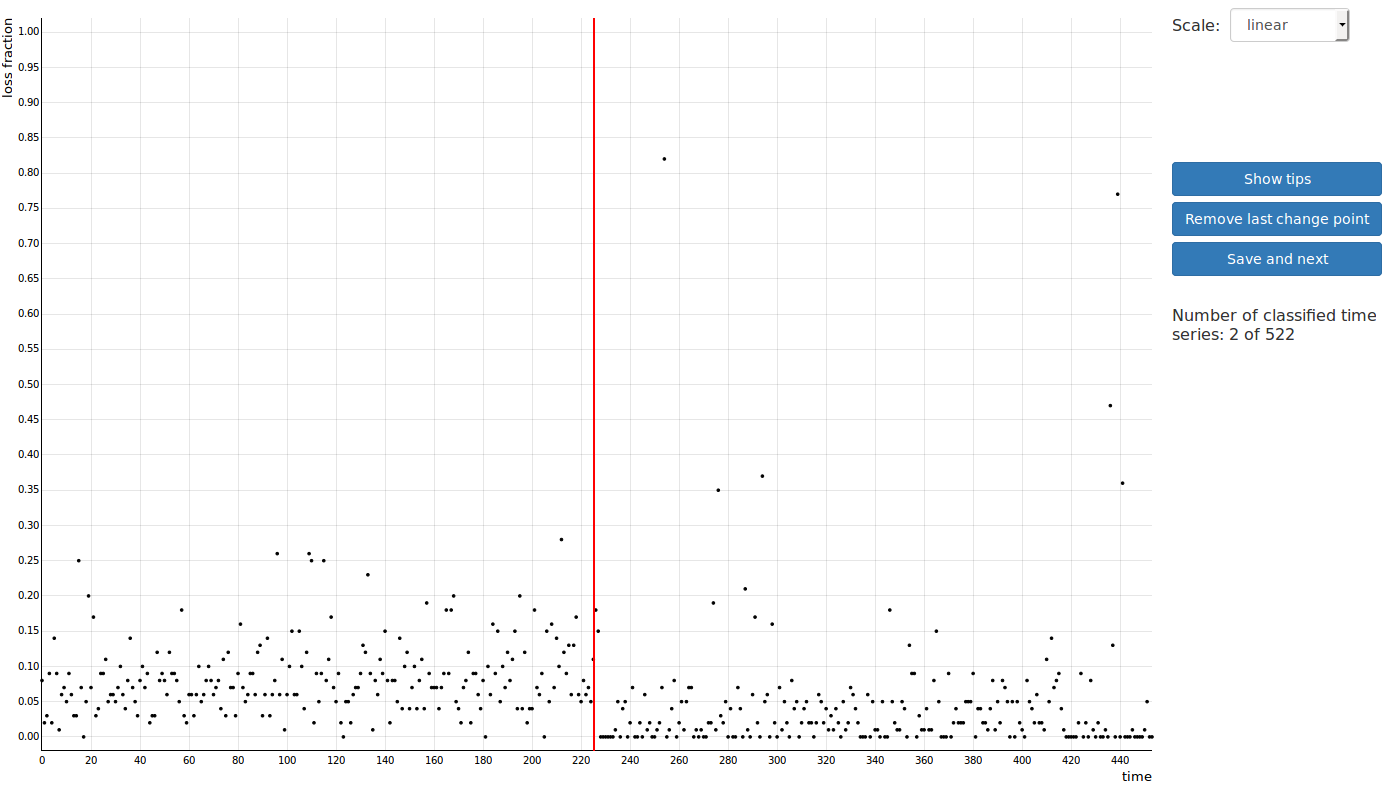
\includegraphics[width=0.9\linewidth]{./figures/methodology/supervised_learning_try/survey_system.png}
    \caption{Survey system snapshot.}
\label{fig:survey_system}
\end{figure}%

Five specialists with experience in network measurements and statistical
modeling, but without background in change point detection, classified Y time
series.
For each time series, the Y classifications were pairwise compared through a
metric of agreement that vary from zero (no agreement) to one (full
agreement). Then is evaluated the average of the agreement of each time series.

The confusion matrix is assessed through the following method. The change
points of one client are represented by

THE ABOVE METRIC IS ASSOCIATIVe?

The change point detection problem can be interpreted as a binary
classification problem in which each point of a time series is classified as
``is a change point'' or ``is not a change point''.
EMPIRICALLY SHOW THE UNBALANCE

Through this analysis looking the different classification patterns it was
defined that this strategy can be noisy, and not reflect real network faults.

It is important to note that the algorithms presented in
Chapter~\ref{chap:change_point_detection} doesn't use a previous point labels
for a training phase. Once a change point dataset is constructed, in which a
train set each labels each point of a time series as a change point or not, can
open new possibilities to a supervised learning procedure, in which are not
much explored in the literature of change pointe detection.

THIS PROCEDURE IMPACT THE MINIMUM/MAXIMUM NUMBER OF CHAGE POINTS TO BE SELECTED
IN THE PIPELINE

\section{Pipeline}

This section describes, in a high level abstraction, the proposed workflow
used to detect network events and localize their cause. When necessary, some
steps are better explored in further sections.
The analysis seeks for events during a specific time period, and considers a
single metric (loss fraction or RTT), which are specified as parameters.
Figure~\ref{fig:pipeline} illustrates the process.

\begin{figure}[H]
    \centering
    \includegraphics[width=0.9\linewidth]{./figures/methodology/pipeline/pipeline.png}
    \caption{Pipeline.}
\label{fig:pipeline}
\end{figure}%

The workflow starts with the End-Users Filtering step,
which aims to remove clients that can negatively affect the analysis.
As an example, this work eliminates clients
that don't have enough measurements, or present
traceroute inconsistencies (in Section~\ref{sec:spatial_correlation}
this issue is better explored).

The Change Point Detection phase preprocess the end-users time series and
identify change points.
Also, the change points are classified in three types of events: failure,
improvement, or inconclusive. For both metrics, a change point defines a
failure event if the average of the window after this point is greater than the
average of the window before. The improvement event is analogous, however is
identified by a mean decrease.
The inconclusive event means that the segments averages are too close.

The Spatial Correlation procedure cluster the end-users in end-groups
according with their location in the network.
This stage must produce a specific grouping structure, which is detailed in
Section~\ref{sec:spatial_correlation}.

The Events Times Correlation aims to combine similar events of different
end-users of an end-group. For example, if three end-users detect a failure at
the same time, this information will be identified in this step. The resulted
grouped events are then named as network events.
The details of this method are clarified in
Section~\ref{sec:events_times_correlation}.

Finally, to localize the events cause, the Spatial-Time Correlation
correlates network events
from different user-groups with the end-groups structure.
This is better exaplained in Section~\ref{sec:spatial_time_correlation}.

\section{Spatial Correlation}
\label{sec:spatial_correlation}

This procedure aims at cluster end-users in end-groups. An end-user can
participate in more than one end-group. To reasons that will be explained in
Session~\ref{sec:spatial_time_correlation} the resulting end-groups structure
must be a tree.

\section{Events Times Correlation}
\label{sec:events_times_correlation}

There are mainly two reasons to detect the same network event, such as an
equipment failure, at different times in different clients. The first one is
related to the fact that the time series are not regularly sampled. The second
one is due to the change point detection algorithm. Therefore, it must be
defined a procedure to, from different clients events, group the events that
are close enough and report them.

In~\cite{troubleshooting_chronic_conditions_in_large_ip_networks, argus_end_to_end_service_anomaly_detection_and_localization_from_an_isps_point_of_view}
the time is transformed in bin, however these works doesn't present how the
co-occurrence is detected, since it is considered a error interval around the
events. Also this strategy introduces discontinuities, since depending no the
data, two points in the same bin can be more distant then points in consecutive
bins. Therefore this work present a different approach.

The idea is an extension of the inexact voting in totally ordered
space~\cite{voting_algorithms}.


\section{Spatial-Time Correlation}
\label{sec:spatial_time_correlation}

\section{Differences to Previous Systems}
